\documentclass[12pt]{article}
\usepackage[utf8]{inputenc}
\usepackage{float}
\usepackage{lipsum}
\usepackage{mwe}
\usepackage{textgreek}
\usepackage[top=1in, bottom=1in, left=1in, right=1in]{geometry}
%\usepackage[margin=1in]{geometry}
\usepackage[onehalfspacing]{setspace}
%\usepackage[doublespacing]{setspace}
\usepackage{hyperref}
\hypersetup{
	colorlinks=true,
	linkcolor=blue,
	filecolor=magenta,      
	urlcolor=cyan,
}
\usepackage{amsmath, amssymb, amsthm}
\usepackage{enumerate, enumitem}
\usepackage{fancyhdr, graphicx, proof, comment, multicol}
\usepackage[none]{hyphenat} % This command prevents hyphenation of words
\binoppenalty=\maxdimen % This command and the next prevent in-line equation breaks
\relpenalty=\maxdimen
%    Good website with common symbols
% http://www.artofproblemsolving.com/wiki/index.php/LaTeX%3ASymbols
%    How to change enumeration using enumitem package
% http://tex.stackexchange.com/questions/129951/enumerate-tag-using-the-alphabet-instead-of-numbers
%    Quick post on headers
% http://timmurphy.org/2010/08/07/headers-and-footers-in-latex-using-fancyhdr/
%    Info on alignat
% http://tex.stackexchange.com/questions/229799/align-words-next-to-the-numbering
% http://tex.stackexchange.com/questions/43102/how-to-subtract-two-equations
%    Text align left-center-right
% http://tex.stackexchange.com/questions/55472/how-to-make-text-aligned-left-center-right-in-the-same-line

\usepackage{microtype} % Modifies spacing between letters and words
\usepackage{mathpazo} % Modifies font. Optional package.
\usepackage{mdframed} % Required for boxed problems.
\usepackage{parskip} % Left justifies new paragraphs.
\linespread{1.1} 

\newcommand{\R}{\mathbb{R}}
\newcommand{\C}{\mathbb{C}}
\newcommand{\Z}{\mathbb{Z}}
\newcommand{\N}{\mathbb{N}}
\newcommand{\Q}{\mathbb{Q}}


\begin{document}
% This is the Header
% Make sure you update this information!!!!

%\noindent
\textbf{Deep Learning Lab (INF.M135)} \hfill \textbf{Marco Ferri} \\
\normalsize Università della Svizzera Italiana \hfill Due Date: 20/12/19 \\

% This is where you name your homework
\begin{center}
\textbf{Assignment 4: Reinforcement Learning}
\end{center}




\section*{Task 1}

\textbf{(10 points) Several Gym wrappers were required to preprocess the data. These wrappers include the \textit{FrameStack} wrapper, the \textit{ScaledFloatFrame} wrapper, the \textit{MaxAndSkipEnv} wrapper, and the \textit{ClipRewardEnv} wrapper. Briefly explain the role of each of these wrappers (in one or two sentences).}

Gym wrappers are used to add features or custom controls around Gym environments in order to modify how data coming from the environment itself should be transformed to handle them in a comfortable way during the learning algorithm. The followings are some of the main wrappers used during the project development:

\begin{itemize}
	\item \textit{FrameStack} is used to stack together a specified amount of Frames, which represent environment observations, and return them altogether as a list of memory-efficient Gym LazyFrames;
	\item \textit{ScaledFloatFrame} is used to rescale Frames (observation) by a value of 255, which so it is useful to represent colors in a [0,1] interval instead of [0,255];
	\item \textit{MaxAndSkipEnv} is used to handle as many sequencial Frames as specified by a given parameter. It modifies the step operation by skipping some Frames and executing the same action on each of them, summing the rewards and returning the maximum over last observations;
	\item \textit{ClipRewardEnv} is simply used to convert reward in a value which is -1, 0 or 1 accordingly to its sign.
\end{itemize}



\section*{Task 2}

\textbf{(10 points) How do Mnih et al. (2015) explain the need for a target Q-network in addition to an online Q- network?}

When a non-linear function (such as a Neural Network) is used to represent the Q-function, Reinforcement Learning is known to be unstable or even to diverge, because of several reasons: the correlation between subsequent observations, Q-values and target values. Also, small changes in the Q-function can lead to policies that get modified too rapidly and inefficiently.

In order to overcome this instability and non-convergence problems, an idea is to break (or reduce) the correlation between Q-values and target by introducing another network  periodically updated and that works together with the online network, which is instead updated step-by-step. This technique is very efficient even for very large networks, and then it represents a good alternative to other known methods in the literature.



\section*{Task 3}

\textbf{(10 points) Why is it necessary to act according to an $\epsilon$-greedy policy instead of a greedy policy (with respect to Q)?}

Reinforcement Learning algorithms are composed of two different phases: exploration and exploitation. While the former is used to allow the agent to explore the state space within the environment, the latter is instead used for improving the agent choices (taken actions) in order to maximize the expected reward.

This process is achieved iteratively by first choosing an action to be taken (using the behavioral policy) and then updating the value function (using the estimation policy) accordingly to the transition just happened. If during the application of behavioral policy, the agent always takes the action which maximizes the expected reward, then the policy is called greedy. The problem with this behavior is that, in this way, the agent is not encouraged to explore new states in case they are worse (in terms of reward) than the already explored ones, and so the algorithm is likely to converge in a local minimum or not converge at all to the optimal policy.

That is why epsilon-greedy policies are introduced in Reinforcement Learning, in order to allow the agent to explore the whole environment by sometimes taking random action, according to a probability which depends on epsilon. The higher the epsilon, the more the possibility for the agent to choose random (and not best) actions. A good algorithm should be able to properly balance exploration and exploitation by acting on the value of epsilon.

More specifically, the Deep Q-Learning algorithm we will use in this project uses an epsilon-greedy behavioral policy and a greedy estimation policy. Since they are different, Q-Learning is called an off-policy algorithm (in contrast with on-policy algorithms, that use the same policy for both behavior and estimation parts).



\clearpage
\section*{Task 4}

\textbf{(50 points) Train your agent as detailed in Section 1.3. You should plot the following metrics in your report: return during training, return during evaluation, TD loss.}

The training has been implemented applying the Deep Q-Learning algorithm with experience replay, as explained in the project description. The main difference with simple Q-Learning, is that DQN tries to approximate the Q function using a Neural Network, which would be a Convolutional Neural Network in this case. CNN allows us to treat states coming from the environment as images, which are the graphical representation of the game at a certain time (what a human gamer actually sees). In this way, the Neural Network behaves not so differently from a human. Observing sequential images, it learns how to infer which is the best action to do in a certain moment, probably understanding under the hood which would be the next position of the ball and how to move accordingly in order to catch it. The whole training is computationally expensive and it has taken around 3 hours and a half using GPU hardware accelerator on Google Colab.

In the following figures, loss and score can be observed. Training score is the sum of all rewards obtained within an episode, computed as moving average over 30 episodes in order to reduce noise. Evaluation score is instead computed every 1000,000 steps by averaging the rewards obtained over 30 different plays (a total of 150 episodes).

Although the loss (temporal difference error) increases through time, the score keeps improving and this means that the network is actually learning. Both from the second and the third figures, it can be seen that better improvements are obtained after the first 1,000,000 steps (out of a total of 2,000,000). Evaluation score, which is the most significative metrics for evaluating the model, reaches a value of around 350 at the last evaluation step and it seems to follow an increasing trend. This result is slightly less than which the state of the art \footnote{"Human-level control through deep reinforcement learning.", \href{https://web.stanford.edu/class/psych209/Readings/MnihEtAlHassibis15NatureControlDeepRL.pdf}{Mnih et al.} (2015)} actually shows for Atari BreakOut using DQN, which should have an evaluation score equal to $401.2 (\pm 26.9)$. Accordingly to Mnhit et al, this is more than 10 times better than what a human can do in the same game.

\begin{figure}[H]
	\centering
	\begin{minipage}{0.49\textwidth}
		\centering
		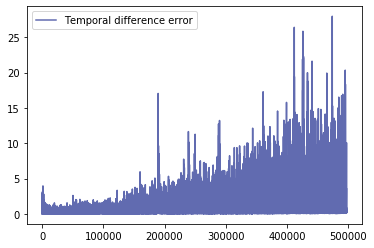
\includegraphics[width=1\textwidth]{images/4_loss.png} % first figure itself
		\caption{Loss over steps}
	\end{minipage}\hfill
	\begin{minipage}{0.49\textwidth}
		\centering
		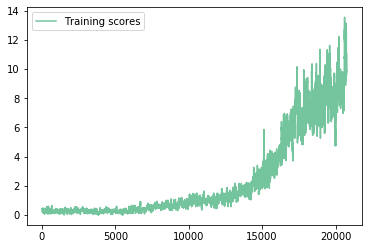
\includegraphics[width=1\textwidth]{images/4_score_train.png} % second figure itself
		\caption{Training score over episodes}
	\end{minipage}
	\label{fig:breakout_loss_trainscore}
\end{figure}

\begin{figure}[H]
	\centering
	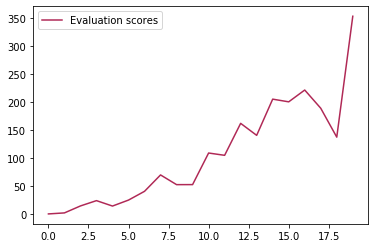
\includegraphics[width=0.65\textwidth]{images/4_score_eval.png} 
	\label{fig:breakout_evalscore}
	\caption{Evaluation score (every 100,000 steps)}
\end{figure}


\section*{Task 5}

\textbf{(10 points) After training, render one episode of interaction between your agent and the environment. For this purpose, you may wrap your environment using a gym.wrappers.Monitor.}

Once the training has been completed, the \textit{Monitor} wrapper has been used to register some games. One of these games is available within this report through an mp4 video file (\texttt{breakout.mp4}), in which it can be seen that the agent is perfectly able to play the game in such a way that overcome human performances, as said in the state of the art.

Please notice that the video shows an entire game (not a single episode), composed of five sequential episodes. Each episode ends when the agent is not able to properly catch the ball - easy to notice if you check the decreasing "remaining lives" on the top of the screen. It can be clearly seen that while the first and second episodes are handled very well by the agent, the next three episodes are very much worse since the agent loses its life very soon. This can mainly happen because of two reasons: once the game proceeds, it becomes harder because the ball gets faster when it touches the last rows of the wall, so the agent finds more difficulties on behaving well; since reaching the end of the game is pretty difficult and it requires several episodes of training for the agent (in order to first learn how to handle the basic of the game itself), it may happen that the episodes in which the agent is asked to compete with difficult challenges (the ones coming from the last wall blocks to be broken) are too few for allowing the agent to learn in a proper way. 

This problem could be handled increasing the number of total episodes used for training the agent or trying to feed the reinforcement learning algorithm with an environment which already simulates last parts of a match, in order to let the agent learn on these situations only, after he learned how to handle first phases of the game.



\section*{Task 6}

\textbf{(10 points) Instead of updating the target network every C = 10000 steps, experiment with C = 50000. Compare in a single plot the average score across evaluations obtained by these two alternatives. How do you explain the differences?}

Training the agent using C=50000 causes the target network to be updated less often than before. The result of this can be seen in the next figure, which shows the comparison between the evalutation score obtained with two different values of C. When C is higher, performances are worse since the maximum score is around 70, compared with a score of about 350 obtained with the previous value of C.

This effect could be explained by considering that a non up-to-date target network can lead to make choices (in terms of action to be taken for the next step in the loss computation) not totally compliant with the knowledge already present in the online network, actually used for calculating the loss which allows to update the network parameters. So, even though the learning is still happening, it results to be slower than usual.

\begin{figure}[H]
	\centering
	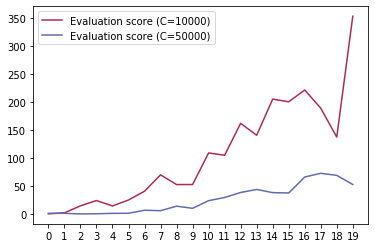
\includegraphics[width=0.65\textwidth]{images/6_score_eval_comparison.png} 
	\label{fig:c_evalscore_comp}
	\caption{Evaluation score comparison (every 100,000 steps)}
\end{figure}



\section*{Task 7}

\textbf{(10 points) Bonus: Repeat the training for a different Atari game.}

Since the code used for performing the training is very generalizable, it can be used for many different games in which the environment follows the same principles as BreakOut does. Given that, running the model with a different Atari game has been very straightforward; the game Centipede has been chosen. An after-training recorded video is available with the report (\texttt{centipede.mp4}), as the previous was. \\
Reference: \url{https://gym.openai.com/envs/Centipede-v0/}

%Watching the video, it can be noticed that also for Centipede the first episodes are handled by the agent better than the last episodes within the same match (each match is composed by three episode).

The following charts show how the agent behaves and even though the game follows different rules for the reward values - so it is not directly comparable with the BreakOut results - it can be seen that the training performances follow the same trend as the previous ones. The last figure shows that, as before, the second half of the episodes executed during the training get the best performance improvements, still having some up and downhills. 

This result is compliant with the finding from the paper "Human-level control through deep reinforcement learning" by Mnih et al., which tells that the evaluation score for Centipede should be $8309 (\pm 5237)$. However, accordingly to the same paper, an agent trained with this method on Centipede performs worse than humans.

\begin{figure}[H]
	\centering
	\begin{minipage}{0.49\textwidth}
		\centering
		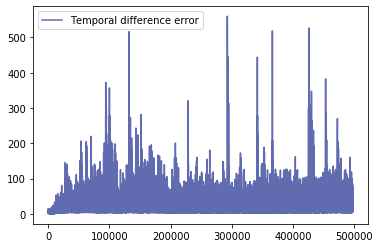
\includegraphics[width=1\textwidth]{images/7_loss.png} % first figure itself
		\caption{Loss over steps}
	\end{minipage}\hfill
	\begin{minipage}{0.49\textwidth}
		\centering
		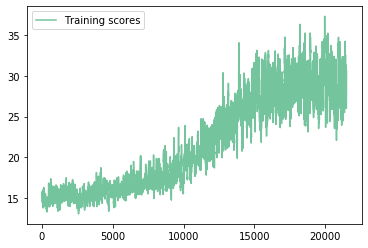
\includegraphics[width=1\textwidth]{images/7_score_train.png} % second figure itself
		\caption{Training score over episodes}
	\end{minipage}
	\label{fig:centipede_loss_trainscore}
\end{figure}

\begin{figure}[H]
	\centering
	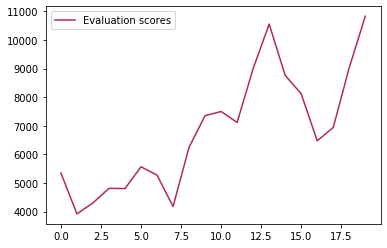
\includegraphics[width=0.65\textwidth]{images/7_score_eval.png} 
	\label{fig:centipede_evalscore}
	\caption{Evaluation score (every 100,000 steps)}
\end{figure}




\end{document}